\documentclass[11pt,a4paper]{article}

\usepackage[margin=0.82in]{geometry}
\usepackage[T1]{fontenc}
\usepackage[utf8]{inputenc}
\usepackage{lmodern}
\usepackage{microtype}
\usepackage{graphicx}
\usepackage{xcolor}
\usepackage{booktabs}
\usepackage{tabularx}
\usepackage{array}
\usepackage{float}
\usepackage{caption}
\usepackage{fancyhdr}
\usepackage[hidelinks]{hyperref}
\usepackage[square,numbers,sort&compress]{natbib}

\hypersetup{
  pdftitle={Phase 1 Concept Proposal},
  pdfauthor={Euriel Chibueze Chukwu}
}

\definecolor{accent}{RGB}{16,78,139}
\definecolor{rulegray}{RGB}{210,215,220}

\setlength{\parindent}{0pt}
\setlength{\parskip}{0.45em}
\setlength{\emergencystretch}{3em}
\renewcommand{\arraystretch}{1.12}
\urlstyle{same}
\raggedbottom

\pagestyle{fancy}
\fancyhf{}
\fancyhead[L]{\small 2026 Global Quantum + AI Challenge | Phase 1 Concept Proposal}
\fancyhead[R]{\small Built 2 Last}
\fancyfoot[C]{\small \thepage}
\renewcommand{\headrulewidth}{0.4pt}
\renewcommand{\footrulewidth}{0pt}
\setlength{\headheight}{14pt}

\newcolumntype{Y}{>{\raggedright\arraybackslash}X}

\begin{document}

\begin{center}
{\Large\bfseries Quantum-Inspired Tensor-Network Finite-Volume Solver for the 2D Convecting Taylor-Green Vortex\par}
\vspace{0.35em}
{\normalsize Enterprise problem statement: efficient PDE solvers for aerodynamic flow simulation\par}
\vspace{0.25em}
{\small 20 May 2026\par}
\end{center}

\vspace{0.4em}
\textcolor{accent}{\rule{\textwidth}{0.8pt}}

\section*{Team's Profile}

\begin{tabularx}{\textwidth}{@{}>{\bfseries}p{0.24\textwidth}Y@{}}
Team name &
Built 2 Last \\
Lead contact details &
Euriel Chibueze Chukwu \\
&
\href{mailto:chukwueuriel@gmail.com}{chukwueuriel@gmail.com} \\
&
+49 1521 4478978 \\
Brief description of each team member &
\textbf{Euriel Chibueze Chukwu} --- team lead, modeling and implementation lead, independent submission team. Euriel holds an M.Sc. in Data Engineering from Constructor University Bremen and a B.Eng. in Mechanical Engineering from the University of Port Harcourt. His relevant expertise combines systems modeling, numerical analysis, fluid systems, data engineering, automation, and technical reporting. Relevant projects from his CV include a master's thesis on assessing the renewable energy potential of Nigeria, a coupled-oscillator synchronization study, and ODE-based dynamic-system modeling of phytoplankton toxin production in a chemostat. \\
Prior experience &
Prior quantum-computing experience is early-stage and project-based rather than formal industrial deployment. The strongest prior background is in the problem domain: engineering mechanics, thermodynamics, fluid systems, mathematical modeling, data analysis, and reproducible technical workflows. This proposal extends that background into quantum-inspired tensor-network compression and benchmarked PDE simulation. \\
\end{tabularx}

\section*{Problem Statement Selection}

This proposal responds to an enterprise problem on scalable PDE solvers for the 2D Convecting Taylor-Green vortex in streamwise flow, using the \textbf{Tensor Network solver within a Finite Volume framework} route named in the challenge brief \cite{ChallengeBrief2025}.

\section*{Abstract}

We present a quantum-inspired tensor-network finite-volume solver for the 2D Convecting Taylor-Green vortex in streamwise flow, aimed at more scalable aerodynamic PDE simulation. The method couples a higher-order MUSCL-TVD finite-volume discretization with tensor-train state compression, randomized truncated-SVD compression kernels, and operator-side compressed transport-state reuse inside the finite-volume update. Benchmarked against the exact analytical solution, a dealiased pseudo-spectral reference, and two classical finite-volume baselines, the current implementation demonstrates a clear memory-efficiency advantage while preserving finite-volume fidelity as Reynolds number increases from \texttt{Re = 10} to \texttt{900}. Relative to the strong uncompressed MUSCL baseline, the compressed solver reduces persistent state memory by \texttt{1.75x} to \texttt{1.99x} while changing relative L2 velocity error by only about \texttt{0.13\%} to \texttt{2.2\%}. The same benchmark also shows a more favorable runtime-growth trend for the compressed solver than for the MUSCL baseline, with fitted runtime-growth exponents of about \texttt{1.24} versus \texttt{1.26}, and absolute runtime wins at \texttt{Re = 300} and \texttt{Re = 600} in the current workstation sweep. The resulting Phase 1 claim is therefore specific and measurable: a working tensor-network finite-volume solver, a validated scaling study, a strong classical comparison stack, and a demonstrated quantum-inspired advantage in memory scaling with a credible path toward stronger end-to-end time-to-solution gains.

\section{Problem Framing}

The target enterprise problem is asking for a PDE-solver path that is both technically credible and materially more scalable than conventional workflows for demanding aerodynamic simulation \cite{ChallengeBrief2025}. For this challenge route, the key question is not whether a quantum-inspired method can be mentioned in the abstract; it is whether the method can be integrated into a finite-volume solver, benchmarked against strong classical baselines, and measured on runtime, memory, and error.

The 2D Convecting Taylor-Green vortex is well suited to that purpose because it has a known analytical solution \cite{TaylorGreen1937}. It lets us separate three things cleanly:

\begin{itemize}
\item fidelity against exact physics;
\item memory cost as the state grows with Reynolds number;
\item time-to-solution growth relative to classical finite-volume baselines.
\end{itemize}

The project therefore frames ``advantage'' narrowly and honestly. The current evidence supports a quantum-inspired memory advantage with strong fidelity retention, plus an improving runtime-scaling trend that is not yet a universal runtime win.

\section{Technical Approach}

The solver stack is intentionally comparative rather than one-off. Four solver tracks are run on the same benchmark:

\begin{table}[H]
\centering
\small
\begin{tabularx}{\textwidth}{@{}p{0.19\textwidth}Y@{}}
\toprule
Track & Role in the benchmark \\
\midrule
\texttt{spectral} & Dealiased pseudo-spectral reference solver, used as the accuracy floor in the classical CFD sense \cite{Orszag1971}. \\
\texttt{fv} & First-order upwind finite-volume baseline, used as the simplest finite-volume comparison point. \\
\texttt{fv-muscl} & Higher-order MUSCL-TVD finite-volume baseline, used as the stronger in-family classical comparator \cite{vanLeer1979,GottliebShu1998}. \\
\texttt{compressed-fv} & Tensor-network-inspired finite-volume solver with tensor-train state compression, randomized low-rank compression kernels \cite{Oseledets2011,HalkoMartinssonTropp2011}, and operator-side compressed transport-state reuse inside the RK update. \\
\bottomrule
\end{tabularx}
\caption{Benchmark stack used to measure advantage against progressively stronger classical references.}
\end{table}

The compressed solver moves beyond post-processing compression. It stores the vorticity state in tensor-train form between steps and reuses a compressed transport-state representation inside the finite-volume update. This makes the compression story relevant to solver execution, not only to archived state size.

The project uses a single acceptance workflow:

\begin{quote}
\texttt{python3 scripts/run\_benchmark.py --solver compare}\\
\texttt{--output-dir results/submission\_core}
\end{quote}

That workflow runs the four solver tracks across \texttt{Re = 10, 100, 300, 600, 900} and records runtime, persistent memory, L2 velocity error, relative kinetic-energy error, and compression behavior in a curated result set.

\section{Feasibility and Resource Requirements}

The current Phase 1 implementation is feasible with standard workstation resources and does not require special hardware:

\begin{itemize}
\item \textbf{Data}: the current benchmark uses the exact analytical Taylor-Green solution as the reference target, so no proprietary enterprise data is required for the Phase 1 claim.
\item \textbf{Compute}: the benchmark runs on a local workstation in Python with NumPy-based solver code and Matplotlib result generation.
\item \textbf{Software}: the repository already contains the solver stack, comparison harness, and curated output artifacts needed to reproduce the main figures and tables.
\item \textbf{Assumptions}: the current evidence is for a 2D canonical vortex benchmark and a single-run workstation sweep. The remaining runtime claim should therefore be interpreted as a scaling trend and partial crossover result, not as a finished industrial runtime win.
\end{itemize}

This is a realistic Phase 1 position: the method is already built and measured, the compute requirements are modest, and the next PoC step is optimization and scaling rather than first implementation.

\section{Expected Impact}

The current results already show why this route is relevant to the target use case. The strongest comparison is between \texttt{fv-muscl} and \texttt{compressed-fv}:

\begin{table}[H]
\centering
\small
\begin{tabular}{@{}rrrr@{}}
\toprule
Re & Memory gain vs MUSCL & Error ratio vs MUSCL & Runtime ratio vs MUSCL \\
\midrule
10  & 1.75x & 1.001x & 1.12x \\
100 & 1.94x & 1.018x & 1.58x \\
300 & 1.97x & 1.022x & 0.86x \\
600 & 1.98x & 1.013x & 0.96x \\
900 & 1.99x & 1.016x & 1.34x \\
\bottomrule
\end{tabular}
\caption{Compressed solver comparison against the stronger finite-volume baseline. Runtime ratios below 1.0 indicate absolute runtime wins in the current sweep.}
\end{table}

Three impact statements follow directly from these measurements:

\begin{itemize}
\item The stronger classical comparison point is meaningful. \texttt{fv-muscl} improves L2 error over the first-order \texttt{fv} baseline by about \texttt{23.6x} to \texttt{354.8x} across the Reynolds sweep.
\item The compressed method preserves that stronger solution closely. Its L2 error changes by only about \texttt{0.13\%} to \texttt{2.2\%} relative to \texttt{fv-muscl}.
\item The compression story scales with state size. Persistent memory reduction improves from \texttt{1.75x} at \texttt{Re = 10} to \texttt{1.99x} at \texttt{Re = 900}.
\end{itemize}

For the target use case, a successful PoC would therefore demonstrate more than a toy compression result. It would show that a tensor-network representation can reduce finite-volume state cost while keeping a strong classical baseline effectively intact.

\section{Validation Plan}

The Phase 2 validation path is already well defined by the current benchmark harness:

\begin{itemize}
\item keep \texttt{--solver compare} as the acceptance test for every compression change;
\item extend the Reynolds and resolution sweep beyond the current \texttt{Re = 900} result;
\item profile runtime, compression share, and operator-compression behavior on the same benchmark;
\item run ablations that switch off structured operator compression or revert to matrix-based state compression;
\item measure success with exact-solution error, persistent memory, runtime ratio versus \texttt{fv-muscl}, and fitted runtime-growth exponents.
\end{itemize}

The current benchmark already defines the central success metric for time-to-solution analysis: how runtime grows with Reynolds number for the compressed solver versus the strongest classical finite-volume baseline. In the curated results, the fitted runtime-growth exponent is about \texttt{1.24} for \texttt{compressed-fv} versus about \texttt{1.26} for \texttt{fv-muscl}, and the compressed solver's runtime growth factor from \texttt{Re = 10} to \texttt{900} is about \texttt{299.3x} versus about \texttt{250.0x} for \texttt{fv-muscl}. That means the current top-end runtime still needs further improvement, but the method is already measurable in the exact way the challenge asks for.

\section{Hybrid / Cross-Domain Integration}

This proposal is hybrid in a practical engineering sense rather than a branding sense. The tensor-network method does not replace the surrounding CFD workflow; it plugs into it:

\begin{itemize}
\item the exact analytical solution remains the physics reference;
\item the pseudo-spectral solver remains the accuracy reference;
\item the higher-order finite-volume solver remains the in-family classical benchmark;
\item the compressed solver reuses the same finite-volume framework, discretization, and validation machinery.
\end{itemize}

That integration path matters for adoption. It means the compression method can be evaluated with the same solver outputs, error metrics, and scaling summaries that classical CFD teams already use. The current implementation is therefore a credible bridge between tensor-network ideas and classical finite-volume engineering practice.

\section{Team Capability}

The team is small but technically aligned to the challenge. Euriel Chibueze Chukwu combines a mechanical-engineering foundation in dynamics, thermodynamics, and fluid systems with postgraduate work in data engineering, modeling, analytics, and reproducible computation. The CV projects most relevant to this submission are the renewable-energy resource modeling thesis, the coupled-oscillator synchronization study, and the ODE-based chemostat model, because they show experience with dynamic-system formulation, numerical analysis, and interpretation of model behavior rather than only software assembly.

The implementation and report preparation were developed with OpenAI Codex assistance under the author's supervision \cite{OpenAICodex2026}. The author set the benchmark objectives, reviewed the generated changes, and validated the reported outputs against the curated result artifacts before inclusion in this submission. That makes the current package suitable for Phase 2 not because it claims completion, but because it already combines a working solver, measured scaling evidence, and a clear next optimization target: turning the improved scaling trend into a stronger and more stable absolute time-to-solution advantage.

\clearpage
\appendix

\section*{Appendix A. Curated Technical Figures}

\begin{figure}[H]
  \centering
  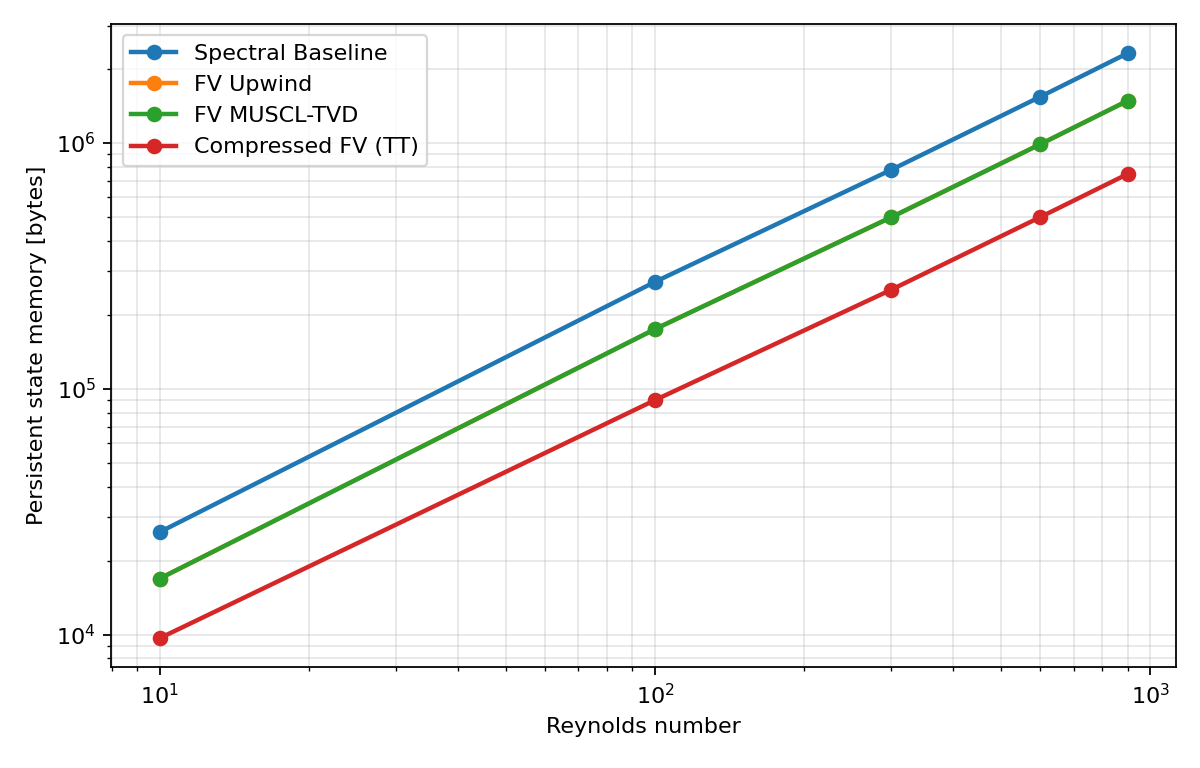
\includegraphics[width=\textwidth,height=0.38\textheight,keepaspectratio]{results/submission_core/comparison_memory_vs_reynolds.png}
  \caption{Persistent state memory versus Reynolds number across the solver tracks.}
\end{figure}

\begin{figure}[H]
  \centering
  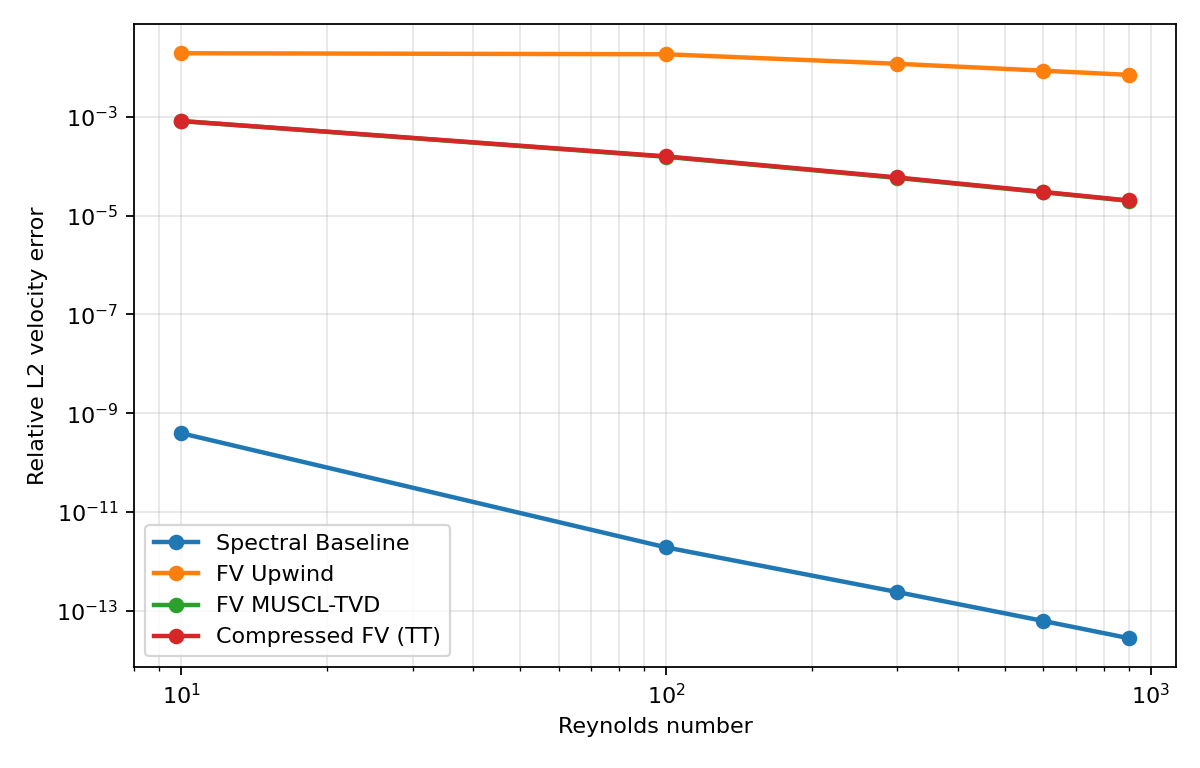
\includegraphics[width=\textwidth,height=0.38\textheight,keepaspectratio]{results/submission_core/comparison_l2_error_vs_reynolds.png}
  \caption{Relative L2 velocity error versus Reynolds number.}
\end{figure}

\clearpage
\section*{Appendix B. Runtime and Tradeoff Evidence}

\begin{figure}[H]
  \centering
  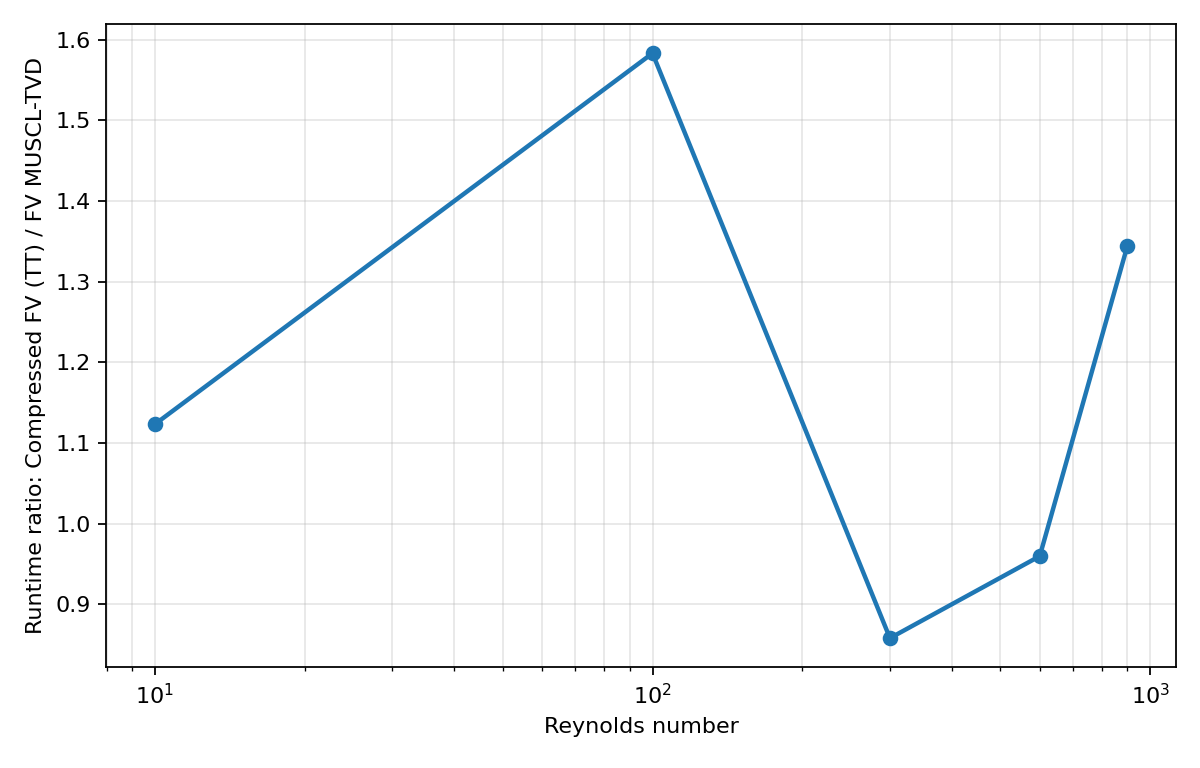
\includegraphics[width=\textwidth,height=0.38\textheight,keepaspectratio]{results/submission_core/comparison_runtime_ratio_vs_reynolds.png}
  \caption{Compressed-to-MUSCL runtime ratio versus Reynolds number.}
\end{figure}

\begin{figure}[H]
  \centering
  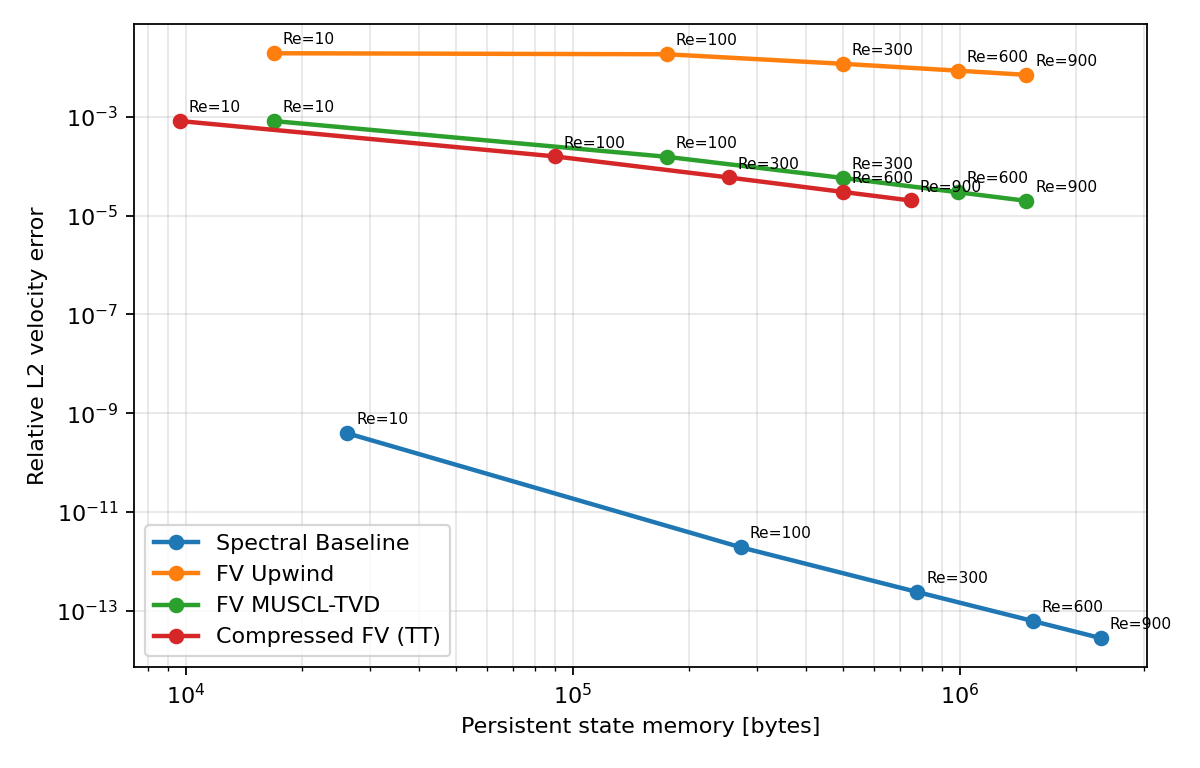
\includegraphics[width=\textwidth,height=0.38\textheight,keepaspectratio]{results/submission_core/comparison_error_vs_memory.png}
  \caption{Memory-versus-fidelity tradeoff across solver tracks.}
\end{figure}

\clearpage
\section*{Appendix C. References}

\begin{thebibliography}{99}

\bibitem{ChallengeBrief2025}
Challenge organizers,
\newblock \emph{Global Quantum Computing Challenge: Challenge Statement},
\newblock enterprise challenge brief, 2025.

\bibitem{TaylorGreen1937}
G. I. Taylor and A. E. Green,
\newblock Mechanism of the production of small eddies from large ones,
\newblock \emph{Proceedings of the Royal Society of London. Series A, Mathematical and Physical Sciences}, 158(895):499--521, 1937.

\bibitem{Orszag1971}
S. A. Orszag,
\newblock On the elimination of aliasing in finite-difference schemes by filtering high-wavenumber components,
\newblock \emph{Journal of the Atmospheric Sciences}, 28(6):1074, 1971.

\bibitem{vanLeer1979}
B. van Leer,
\newblock Towards the ultimate conservative difference scheme. V. A second-order sequel to Godunov's method,
\newblock \emph{Journal of Computational Physics}, 32(1):101--136, 1979.

\bibitem{GottliebShu1998}
S. Gottlieb and C.-W. Shu,
\newblock Total variation diminishing Runge-Kutta schemes,
\newblock \emph{Mathematics of Computation}, 67(221):73--85, 1998.

\bibitem{Oseledets2011}
I. V. Oseledets,
\newblock Tensor-train decomposition,
\newblock \emph{SIAM Journal on Scientific Computing}, 33(5):2295--2317, 2011.

\bibitem{HalkoMartinssonTropp2011}
N. Halko, P. G. Martinsson, and J. A. Tropp,
\newblock Finding structure with randomness: Probabilistic algorithms for constructing approximate matrix decompositions,
\newblock \emph{SIAM Review}, 53(2):217--288, 2011.

\bibitem{OpenAICodex2026}
OpenAI,
\newblock \emph{Codex Workflows},
\newblock official product documentation, \url{https://developers.openai.com/codex/workflows}, accessed May 20, 2026.

\end{thebibliography}

\end{document}
